\begin{frame}
\frametitle{Volumetric Features}
\begin{columns}[c]
\column{0.33\textwidth}
A number of features were used for pattern recognition.

Firstly, two features relating to relative volumes.

Initial velocity divergence is similar to logarithms of Jacobian determinants.
\column{0.33\textwidth}
Jacobian Determinants

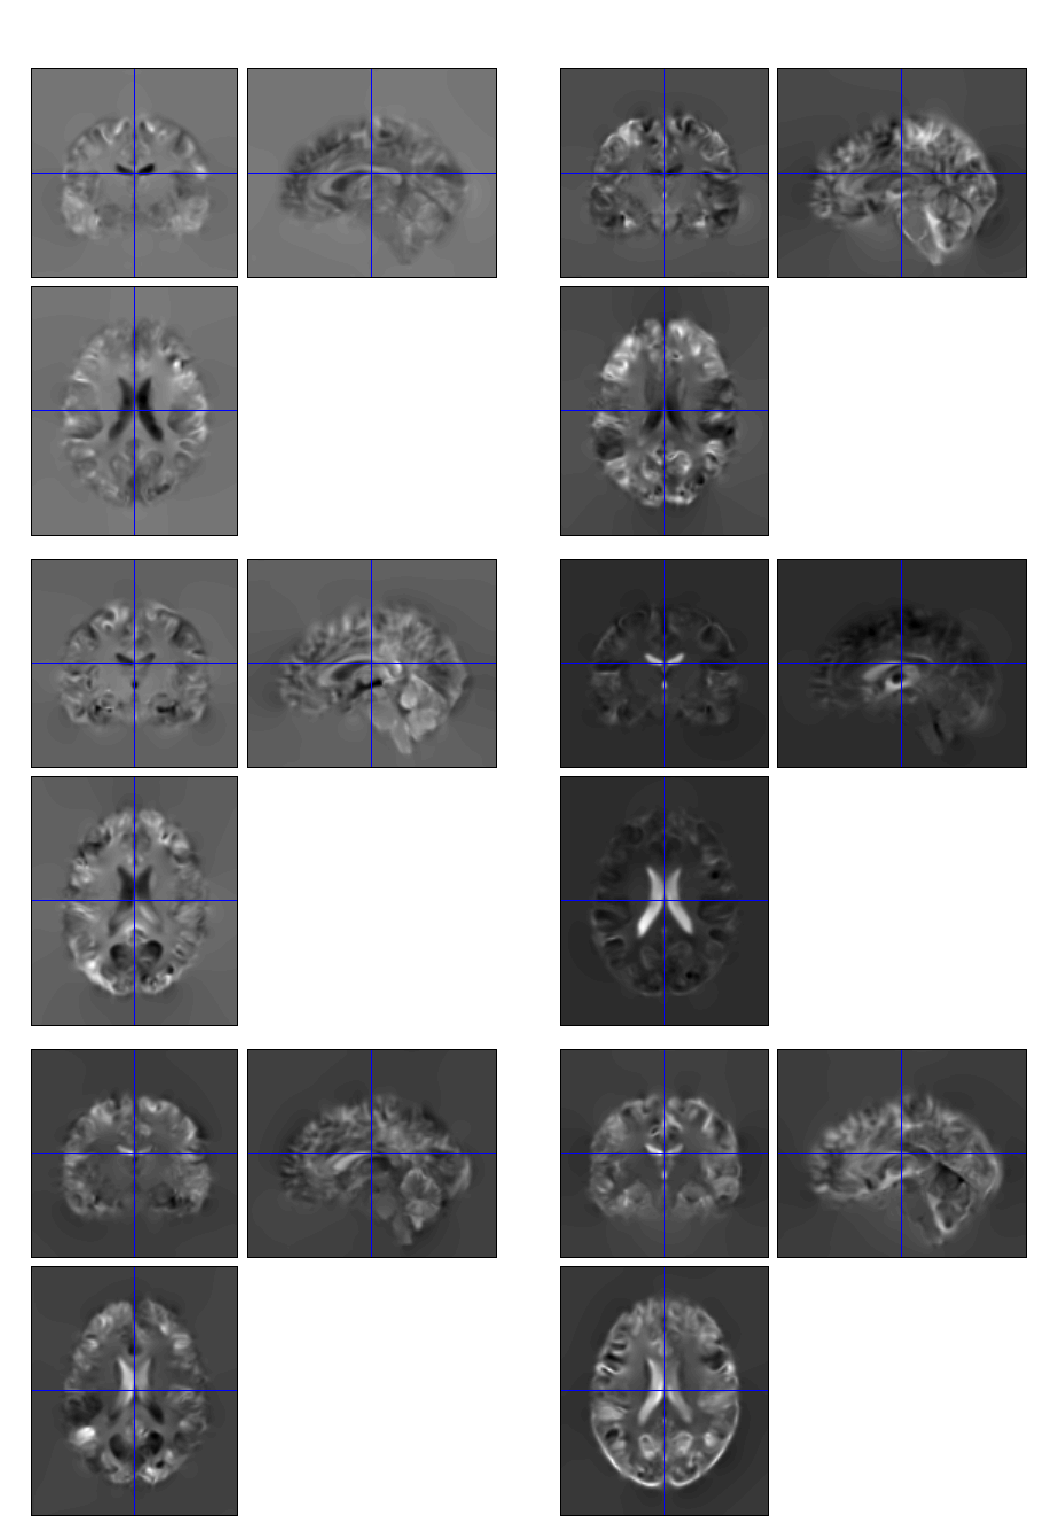
\includegraphics[width=1\textwidth]{jac_ixi}
\column{0.33\textwidth}
Initial Velocity Divergence
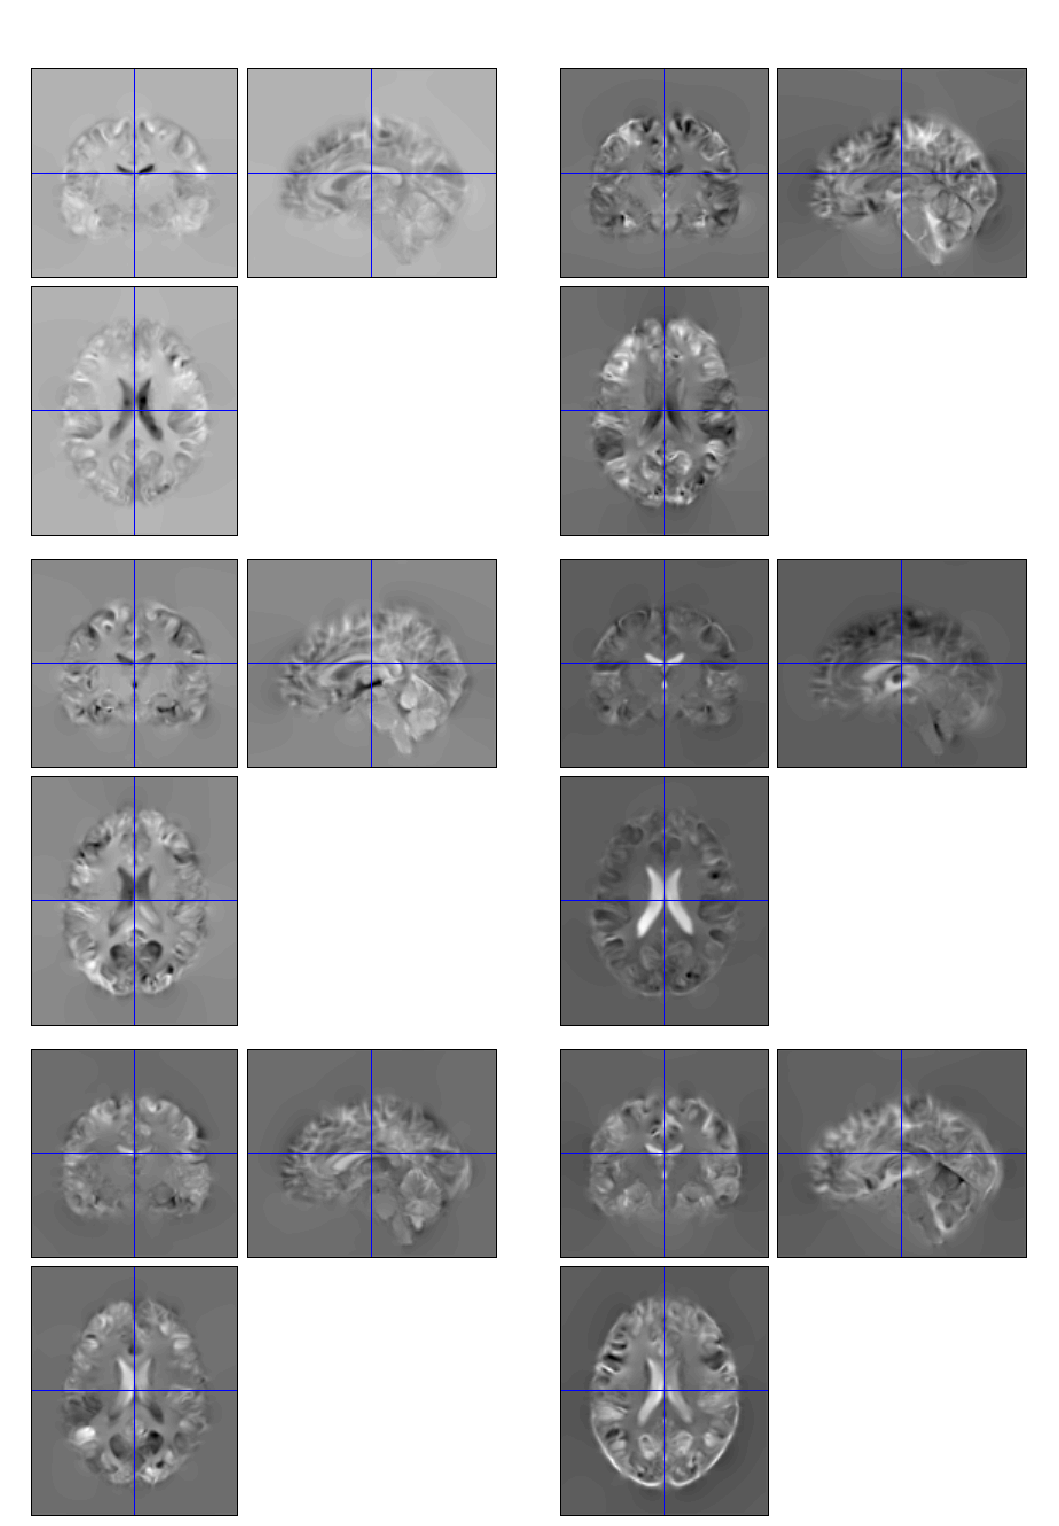
\includegraphics[width=1\textwidth]{div_ixi}
\end{columns}
\end{frame}

%%%%%%%%%%%%%%%%%%%%%%%%%%%%%%%%%%%%%%%%%%%%%%%%%%%%%%%%%%%%%%%
\begin{frame}
\frametitle{Grey Matter Features}
\begin{columns}[c]
\column{0.33\textwidth}
Rigidly Registered GM

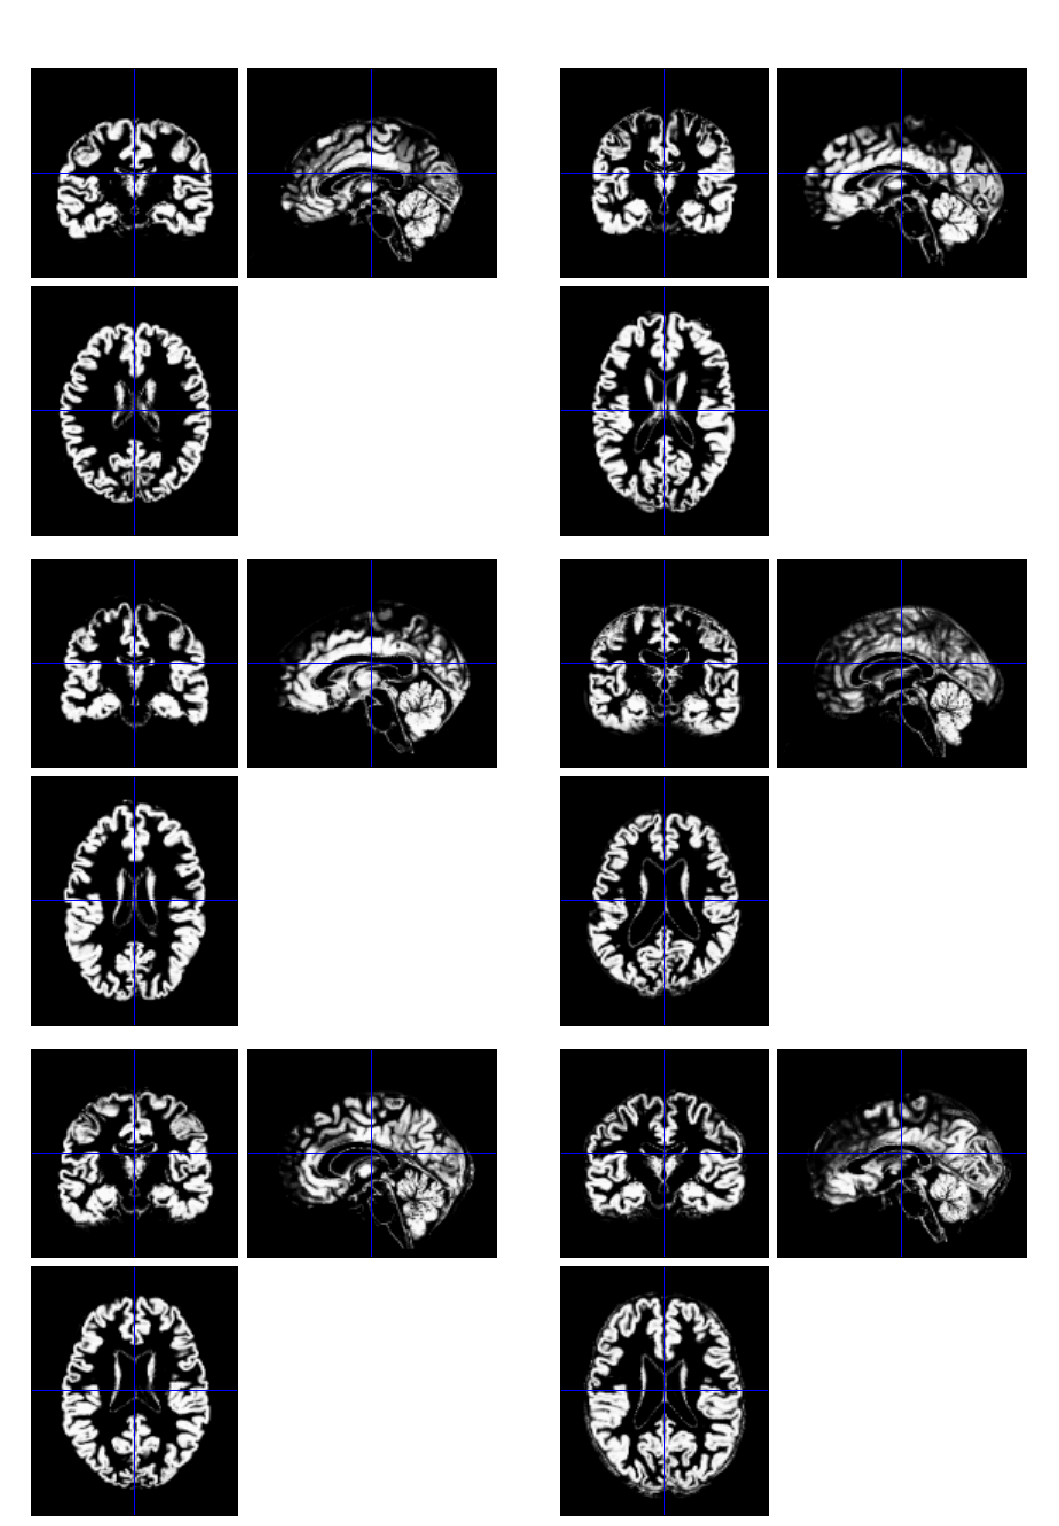
\includegraphics[width=1\textwidth]{gm_ixi}

\column{0.33\textwidth}
Nonlinearly Registered GM

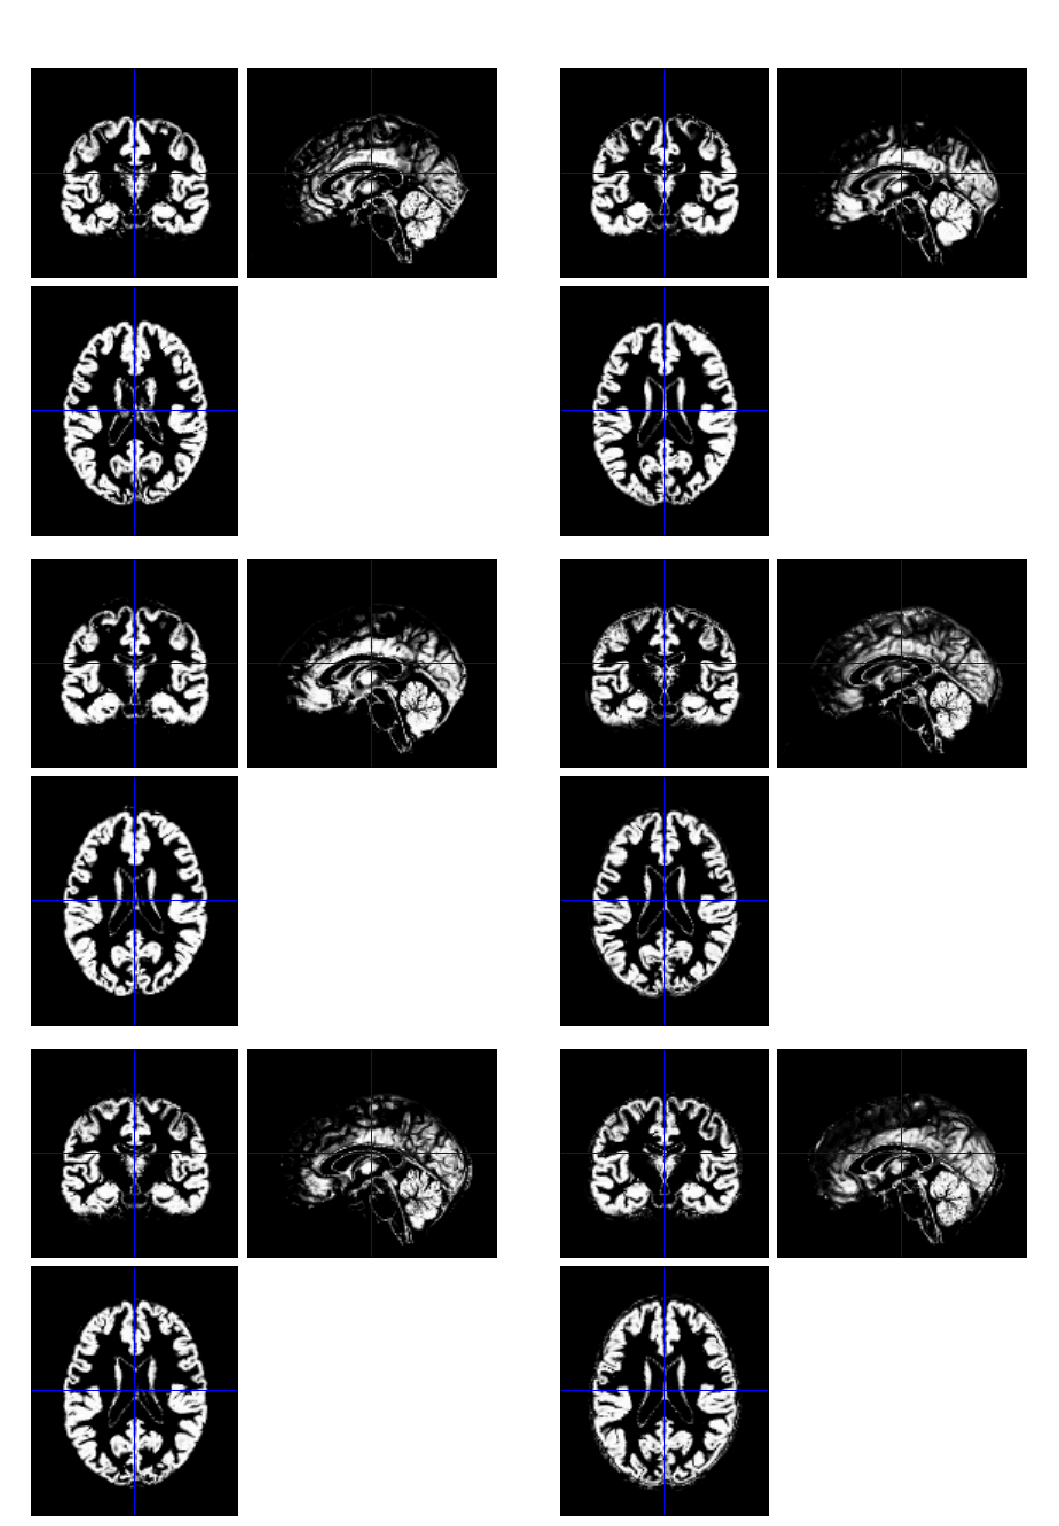
\includegraphics[width=1\textwidth]{wc1_ixi}
\column{0.33\textwidth}
Registered and Jacobian Scaled GM

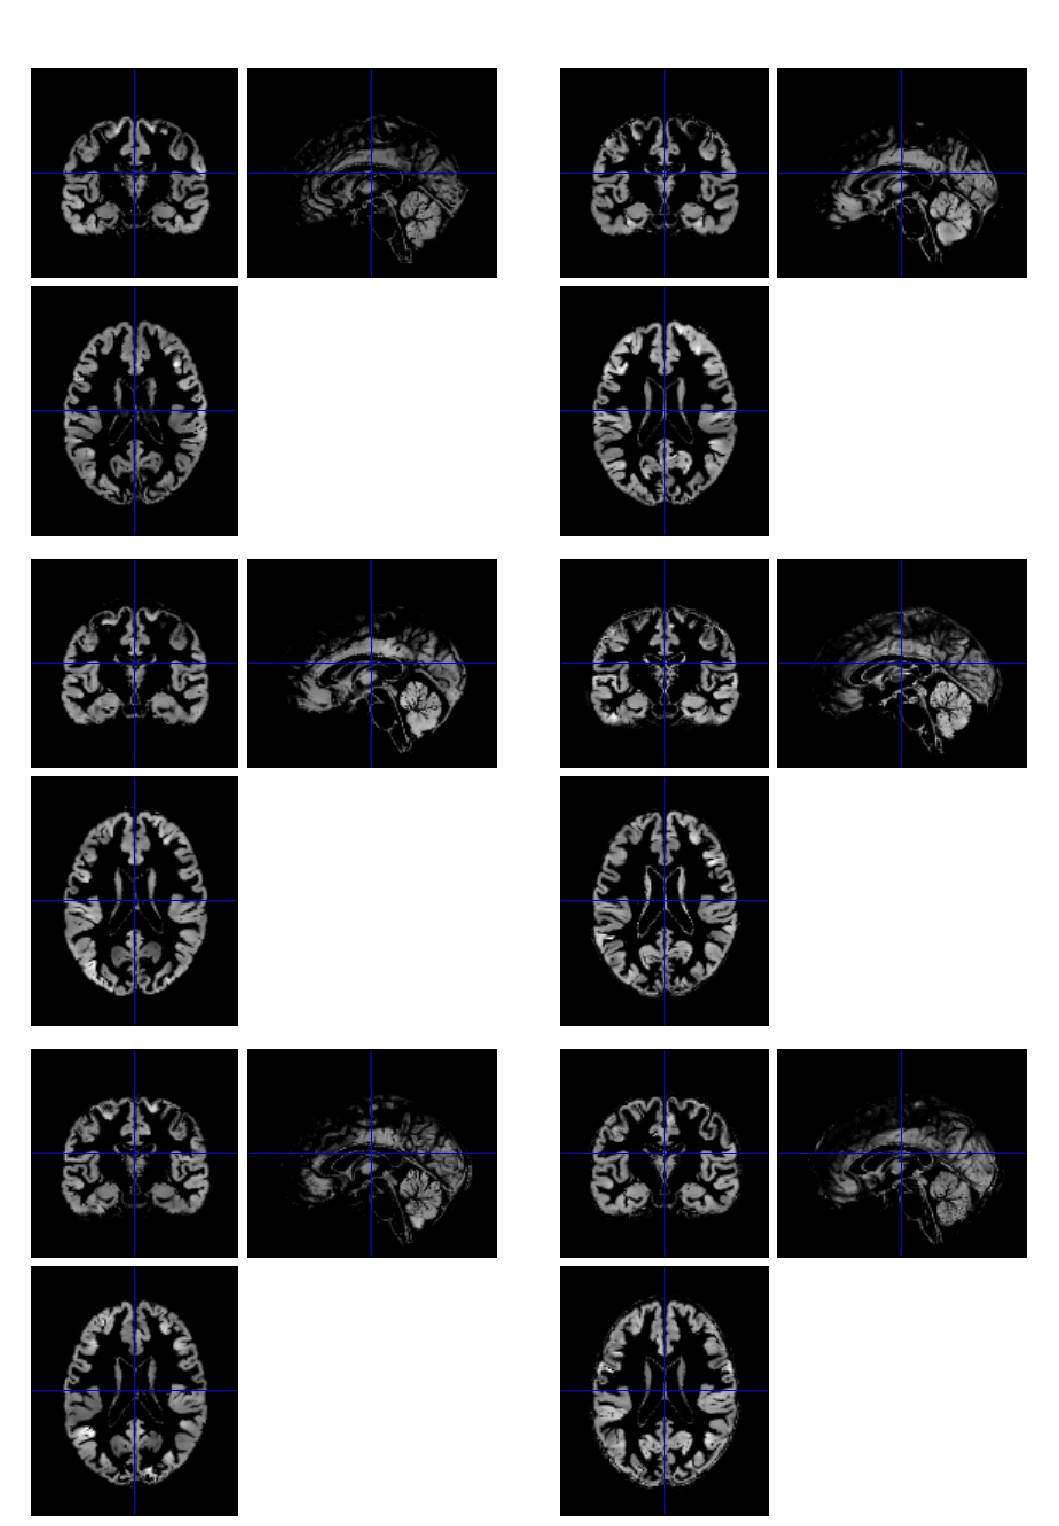
\includegraphics[width=1\textwidth]{mwc1_ixi}
\end{columns}
\end{frame}

%%%%%%%%%%%%%%%%%%%%%%%%%%%%%%%%%%%%%%%%%%%%%%%%%%%%%%%%%%%%%%%
%%%%%%%%%%%%%%%%%%%%%%%%%%%%%%%%%%%%%%%%%%%%%%%%%%%%%%%%%%%%%%%
\begin{frame}
\frametitle{``Scalar Momentum'' Features}
\begin{columns}[c]
\column{0.33\textwidth}
``Scalar momentum'' actually has two components because GM was matched with GM and WM was matched with WM.
\column{0.33\textwidth}
First Momentum Component

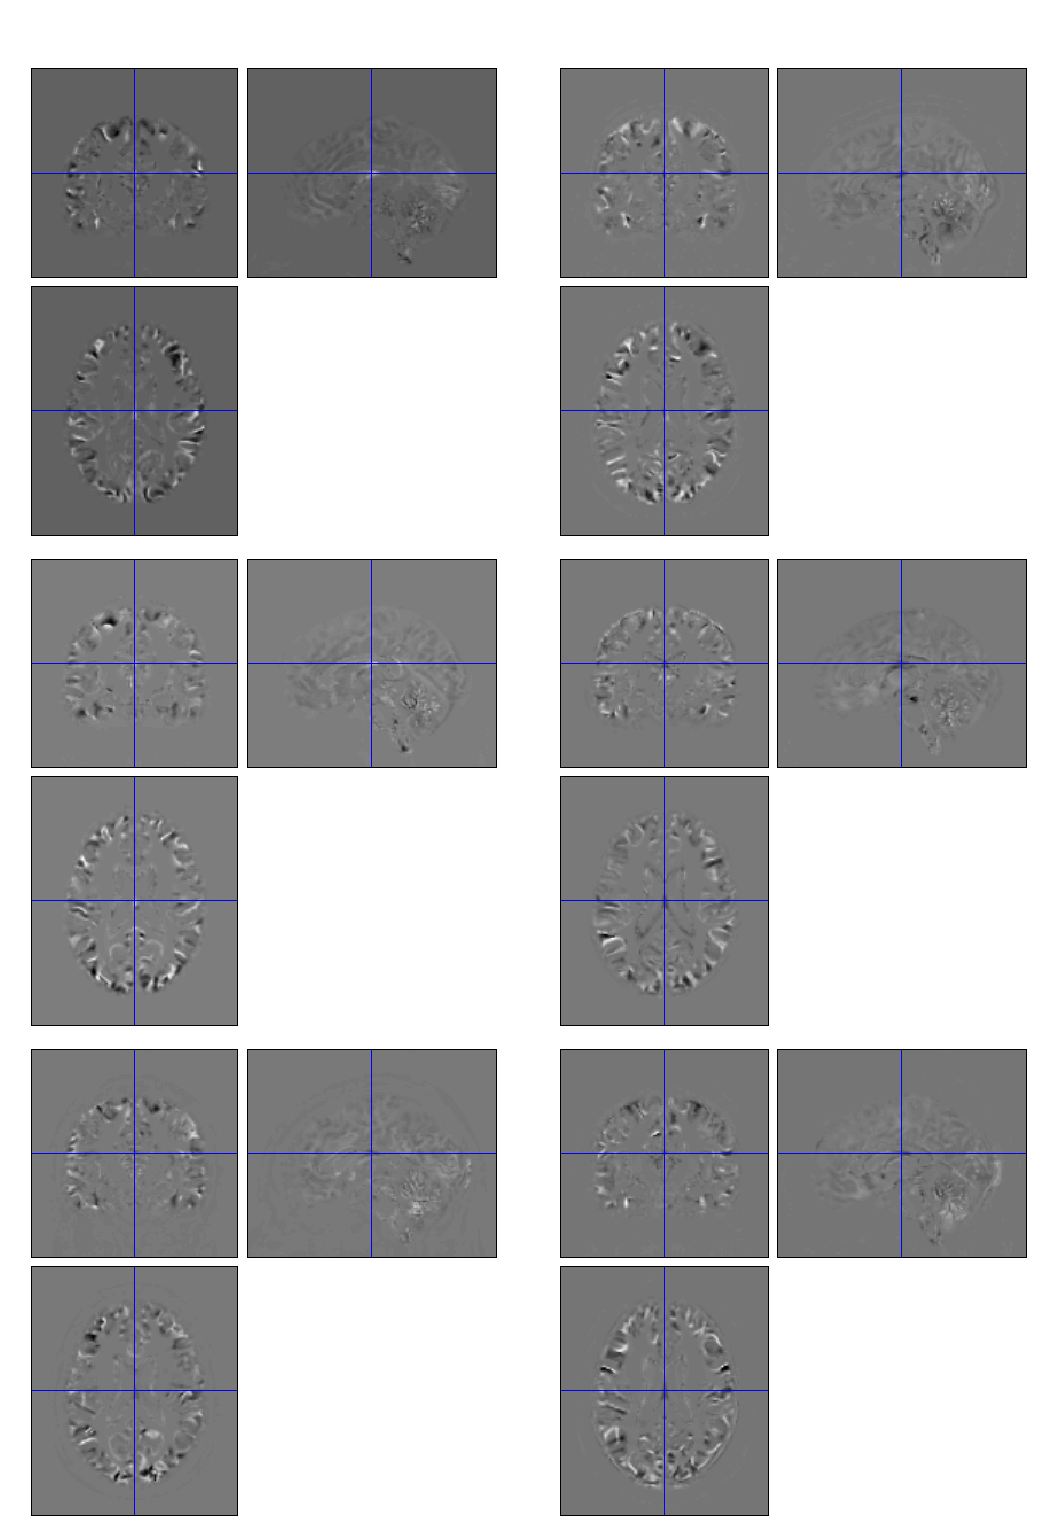
\includegraphics[width=1\textwidth]{resids1_ixi}
\column{0.33\textwidth}
Second Momentum Component

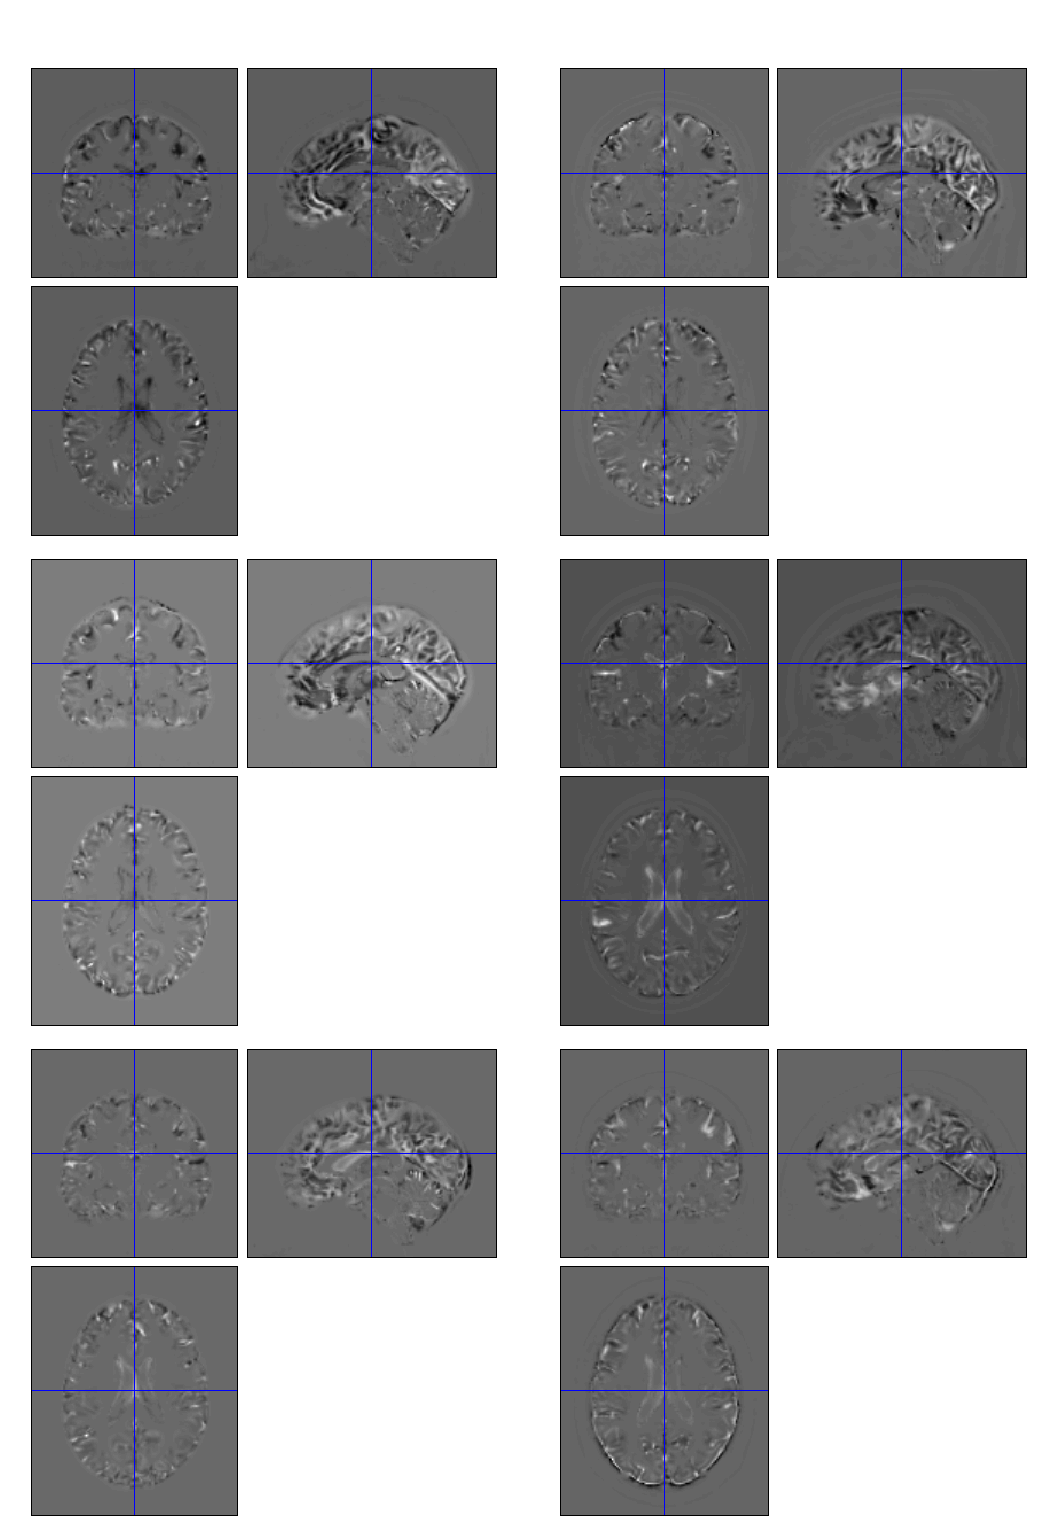
\includegraphics[width=1\textwidth]{resids2_ixi}
\end{columns}
\end{frame}


